\section{Experimental results}

\subsection{Simple function task}

Our simple function task samples an input vector $\mathbf{x}$ from a uniform distribution. From this input vector, the sum of two subsets $a$ and $b$ are then computed. Finally the target $t$ is then an operation performed on $a$ and $b$ (e.g. $a \cdot b$). This is identical to the task by the same name in the Original NALU paper \cite{trask-nalu}. Except that we parameterize it in order to compare the models for different configurations, see figure \ref{fig:simple-function-task-problem}. To make comparison simple, we define a set of default parameters (table \ref{tab:simple-function-task-defaults}) and only vary one of them at the time.

\begin{figure}[H]
\centering
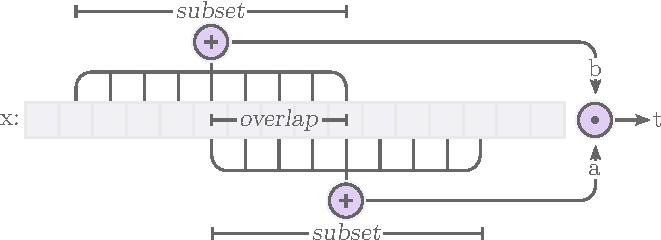
\includegraphics[scale=0.8]{graphics/function_task_static_problem.pdf}
\caption{Dataset is parameterized into ``Input Size'', ``Subset Ratio'', ``Overlap Ratio'', an Operation (here showing multiplication), ``Interpolation Range'' and ``Extrapolation Range'' from which the data set sampled.}
\label{fig:simple-function-task-problem}
\end{figure}

\begin{table}[H]
\caption{Default dataset parameters}
\label{tab:simple-function-task-defaults}
\centering
\begin{tabular}{r l}
\toprule
 Parameter Name & Default Value \\
 \midrule
 Input Size & 100 \\
 Subset Ratio & 0.25 \\
 Overlap Ratio & 0.5 \\
 Interpolation Range & $U[1,2]$ \\
 Extrapolation Range & $U[1,6]$ \\
 \bottomrule
\end{tabular}
\end{table}

Normally one would report the interpolation and extrapolation loss. However, complex approximations that one would typically see in neural networks are not considered good enough. The goal is to achieve a solution that is sufficiently close to a perfect solution. Because there can be many valid permutations of a perfect solution, especially for addition, a solution is judged firsts on the final extrapolation error, and then on a sparsity error.



\subsubsection{Very simple function}

To empirically validate the theoretical problems with $\mathrm{NAC}_{\bullet}$, let's consider the very simple problem shown earlier in figure \ref{fig:nac-mul-eps-issue}. That is $x \in \mathbb{R}^4$, $a = x_1 + x_2$ and $b = x_1 + x_2 + x_3 + x_4$. The solution to this problem is that seen in equation \ref{eq:very-simple-function-ideal-solution}.
\begin{equation}
    \mathbf{W}_1 = \begin{bmatrix}
    1 & 1 & 0 & 0 \\
    1 & 1 & 1 & 1
    \end{bmatrix}, \mathbf{W}_2 = \begin{bmatrix}
    1 & 1
    \end{bmatrix}
    \label{eq:very-simple-function-ideal-solution}
\end{equation}

Each model is trained 100 times with different seeds, and stopped after 200000 iterations. The results (table \ref{tab:very-simple-function-results}), shows that NMU have a much higher success rate and converges much faster. The few cases that did not converge successfully are because of underflow when exactly 0 is multiplied.


In this case the model is considered 

\begin{table}[!h]

\caption{\label{tab:very-simple-function-results}Shows the success-rate, at what global step the model converged at, and the sparsity error for all weight matrices, with 95\% confidence interval. Best result is highlighed.}
\centering
\begin{tabular}{crllll}
\toprule
\multicolumn{1}{c}{Op} & \multicolumn{1}{c}{Model} & \multicolumn{1}{c}{Success} & \multicolumn{2}{c}{Solved at} & \multicolumn{1}{c}{Sparsity error} \\
\cmidrule(l{3pt}r{3pt}){1-1} \cmidrule(l{3pt}r{3pt}){2-2} \cmidrule(l{3pt}r{3pt}){3-3} \cmidrule(l{3pt}r{3pt}){4-5} \cmidrule(l{3pt}r{3pt}){6-6}
 &  & Rate & Median & Mean & Mean\\
\midrule
 & $\mathrm{NAC}_{\bullet}$ & $13\% {~}^{+8\%}_{-5\%}$ & $5.5 \cdot 10^{4}$ & $5.9 \cdot 10^{4} {~}^{+7.8 \cdot 10^{3}}_{-6.6 \cdot 10^{3}}$ & $7.5 \cdot 10^{-6} {~}^{+2.0 \cdot 10^{-6}}_{-2.0 \cdot 10^{-6}}$\\

 & NALU & $26\% {~}^{+9\%}_{-8\%}$ & $7.0 \cdot 10^{4}$ & $7.8 \cdot 10^{4} {~}^{+6.2 \cdot 10^{3}}_{-8.6 \cdot 10^{3}}$ & $9.2 \cdot 10^{-6} {~}^{+1.7 \cdot 10^{-6}}_{-1.7 \cdot 10^{-6}}$\\

\multirow{-3}{*}{\centering\arraybackslash $\bm{\times}$} & NMU & $\mathbf{94\%} {~}^{+3\%}_{-6\%}$ & $\mathbf{1.4 \cdot 10^{4}}$ & $\mathbf{1.4 \cdot 10^{4}} {~}^{+2.2 \cdot 10^{2}}_{-2.1 \cdot 10^{2}}$ & $\mathbf{2.6 \cdot 10^{-8}} {~}^{+6.4 \cdot 10^{-9}}_{-6.4 \cdot 10^{-9}}$\\
\bottomrule
\end{tabular}
\end{table}


\subsubsection{Static function task - defaults}
\begin{table}[!h]

\caption{\label{tab:function-task-static-defaults}Shows the success-rate for $\mathcal{L}_{\mathbf{W}_1, \mathbf{W}_2} < \mathcal{L}_{\mathbf{W}_1^\epsilon, \mathbf{W}_2^*}$, at what global step the model converged at, and the sparsity error for all weight matrices.}
\centering
\begin{tabular}{crllll}
\toprule
\multicolumn{1}{c}{Op} & \multicolumn{1}{c}{Model} & \multicolumn{1}{c}{Success} & \multicolumn{2}{c}{Solved at} & \multicolumn{1}{c}{Sparsity error} \\
\cmidrule(l{3pt}r{3pt}){1-1} \cmidrule(l{3pt}r{3pt}){2-2} \cmidrule(l{3pt}r{3pt}){3-3} \cmidrule(l{3pt}r{3pt}){4-5} \cmidrule(l{3pt}r{3pt}){6-6}
 &  & Rate & Median & Mean & Mean\\
\midrule
 & $\mathrm{NAC}_{\bullet}$ & $30\%$ & $2.5 \cdot 10^{6}$ & $2.5 \cdot 10^{6} \pm 1.5 \cdot 10^{6}$ & $\mathbf{3.9 \cdot 10^{-4} \pm 9.4 \cdot 10^{-4}}$\\

 & Linear & $0\%$ & --- & --- & ---\\

 & NALU & $0\%$ & --- & --- & ---\\

\multirow{-4}{*}{\centering\arraybackslash $\bm{\times}$} & NMU & $\mathbf{90\%}$ & $\mathbf{1.4 \cdot 10^{6}}$ & $\mathbf{1.6 \cdot 10^{6} \pm 5.6 \cdot 10^{5}}$ & $1.8 \cdot 10^{-3} \pm 1.1 \cdot 10^{-3}$\\
\cmidrule{1-6}
 & $\mathrm{NAC}_{+}$ & $\mathbf{100\%}$ & $6.0 \cdot 10^{4}$ & $7.1 \cdot 10^{4} \pm 2.4 \cdot 10^{4}$ & $4.8 \cdot 10^{-1} \pm 2.0 \cdot 10^{-2}$\\

 & Linear & $\mathbf{100\%}$ & $4.2 \cdot 10^{4}$ & $\mathbf{4.2 \cdot 10^{4} \pm 1.9 \cdot 10^{3}}$ & $6.1 \cdot 10^{-1} \pm 1.2 \cdot 10^{-1}$\\

 & NALU & $0\%$ & --- & --- & ---\\

\multirow{-4}{*}{\centering\arraybackslash $\bm{+}$} & NAU & $\mathbf{100\%}$ & $\mathbf{1.8 \cdot 10^{4}}$ & $7.0 \cdot 10^{5} \pm 9.2 \cdot 10^{5}$ & $\mathbf{1.7 \cdot 10^{-3} \pm 8.0 \cdot 10^{-4}}$\\
\cmidrule{1-6}
 & $\mathrm{NAC}_{+}$ & $\mathbf{100\%}$ & $8.0 \cdot 10^{3}$ & $1.5 \cdot 10^{6} \pm 1.5 \cdot 10^{6}$ & $4.6 \cdot 10^{-1} \pm 2.9 \cdot 10^{-2}$\\

 & Linear & $\mathbf{100\%}$ & $1.1 \cdot 10^{6}$ & $1.9 \cdot 10^{6} \pm 1.3 \cdot 10^{6}$ & $3.7 \cdot 10^{-1} \pm 1.1 \cdot 10^{-1}$\\

 & NALU & $20\%$ & $3.6 \cdot 10^{6}$ & $3.6 \cdot 10^{6} \pm 1.3 \cdot 10^{7}$ & $4.7 \cdot 10^{-1} \pm 3.3 \cdot 10^{-1}$\\

\multirow{-4}{*}{\centering\arraybackslash $\bm{-}$} & NAU & $\mathbf{100\%}$ & $\mathbf{4.0 \cdot 10^{3}}$ & $\mathbf{4.2 \cdot 10^{3} \pm 3.0 \cdot 10^{2}}$ & $\mathbf{1.9 \cdot 10^{-3} \pm 4.2 \cdot 10^{-4}}$\\
\bottomrule
\end{tabular}
\end{table}


\subsubsection{Static function task - boundary}
\begin{figure}[H]
\centering
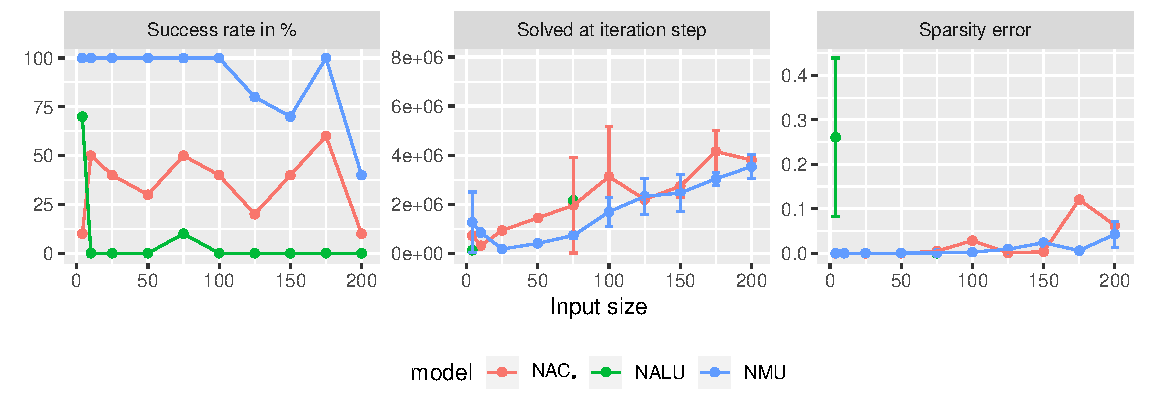
\includegraphics[width=\linewidth]{results/simple_function_static_input_size.pdf}
\caption{Lorem Ipsum.}
\end{figure}

\begin{figure}[H]
\centering
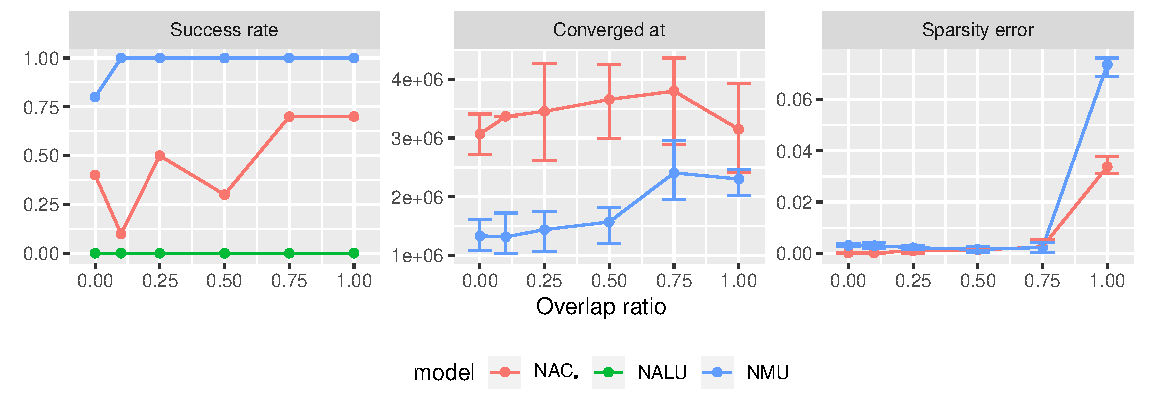
\includegraphics[width=\linewidth]{results/simple_function_static_overlap.pdf}
\caption{Lorem Ipsum.}
\end{figure}

\begin{figure}[H]
\centering
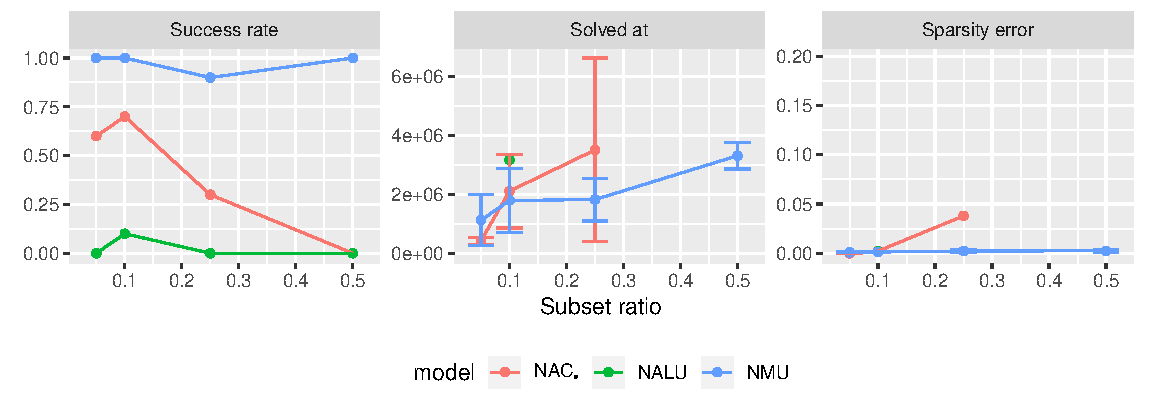
\includegraphics[width=\linewidth]{results/simple_function_static_subset.pdf}
\caption{Lorem Ipsum.}
\end{figure}

\subsection{sequential MNIST}

\begin{figure}[H]
\centering
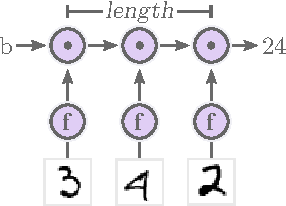
\includegraphics[scale=1]{graphics/mnist_sequence_problem.pdf}
\caption{Lorem Ipsum.}
\end{figure}

